\documentclass[11pt,a4paper]{article}

\usepackage[utf8]{inputenc}
\usepackage[T1]{fontenc}
\usepackage{lmodern}
\usepackage[a4paper,margin=2cm]{geometry}
\usepackage{graphicx}
\usepackage{booktabs}
\usepackage{hyperref}
\usepackage{float}
\usepackage{subcaption}
\usepackage{titlesec}
\usepackage{fancyhdr}

\titlespacing*{\section}{0pt}{1.0em}{0.5em}
\titlespacing*{\subsection}{0pt}{0.7em}{0.35em}

\pagestyle{fancy}
\fancyhf{}
\lhead{Autonomous Systems}
\rhead{Susanna Ardig\`o}
\cfoot{\thepage}

\title{Autonomous Systems}
\author{Susanna Ardig\`o}
\date{Due: May 31 2026}

\begin{document}

\maketitle

\section{Introduction}

This project analyzes an autonomous systems dataset using graph-based methods. Starting from a computer-server connection matrix, the data is transformed into weighted graphs to study influential nodes, communities, cliques, and heavy hitters.

The notebook contains the full implementation and output. This report summarizes the main choices and observations.

\section{Implementation Note}

The analysis was first developed in a Python script and then transferred to a notebook. The code follows an object-oriented structure: each graph representation is handled by a dedicated class, while a higher-level data class coordinates the workflow.

\section{Data Exploration and Graph Construction}

\subsection{Original Dataset}

The dataset is a binary connection matrix: rows represent computers, columns represent servers, and each entry indicates whether a connection exists.

During loading, empty rows and columns are removed because they do not contribute meaningful information to the projected graphs. Basic statistics and the cleaned matrix visualization are provided in the notebook, while Figure~\ref{fig:matrices} gives a compact view of the original matrix and the two projections.

\subsection{Graph Projections}

Since rows and columns represent different entity types, two weighted graph projections are constructed. The computer graph links computers sharing at least one server; the server graph links servers sharing at least one computer.

The edge weight is the number of shared connections, preserving the strength of each relationship. Figure~\ref{fig:original-matrix} shows the original matrix, while Figures~\ref{fig:computer-adjacency} and~\ref{fig:server-adjacency} show the two projected adjacency matrices.

\begin{figure}[h]
    \centering
    \begin{subfigure}{0.18\textwidth}
        \centering
        
\includegraphics[height=0.24\textheight]{../res/Heatmap_connections.png}
        \caption{Original matrix.}
        \label{fig:original-matrix}
    \end{subfigure}
    \hfill
    \begin{subfigure}{0.38\textwidth}
        \centering
        \includegraphics[height=0.24\textheight]{../res/Adjacency_Matrix_Computers.png}
        \caption{Computer projection.}
        \label{fig:computer-adjacency}
    \end{subfigure}
    \hfill
    \begin{subfigure}{0.38\textwidth}
        \centering
        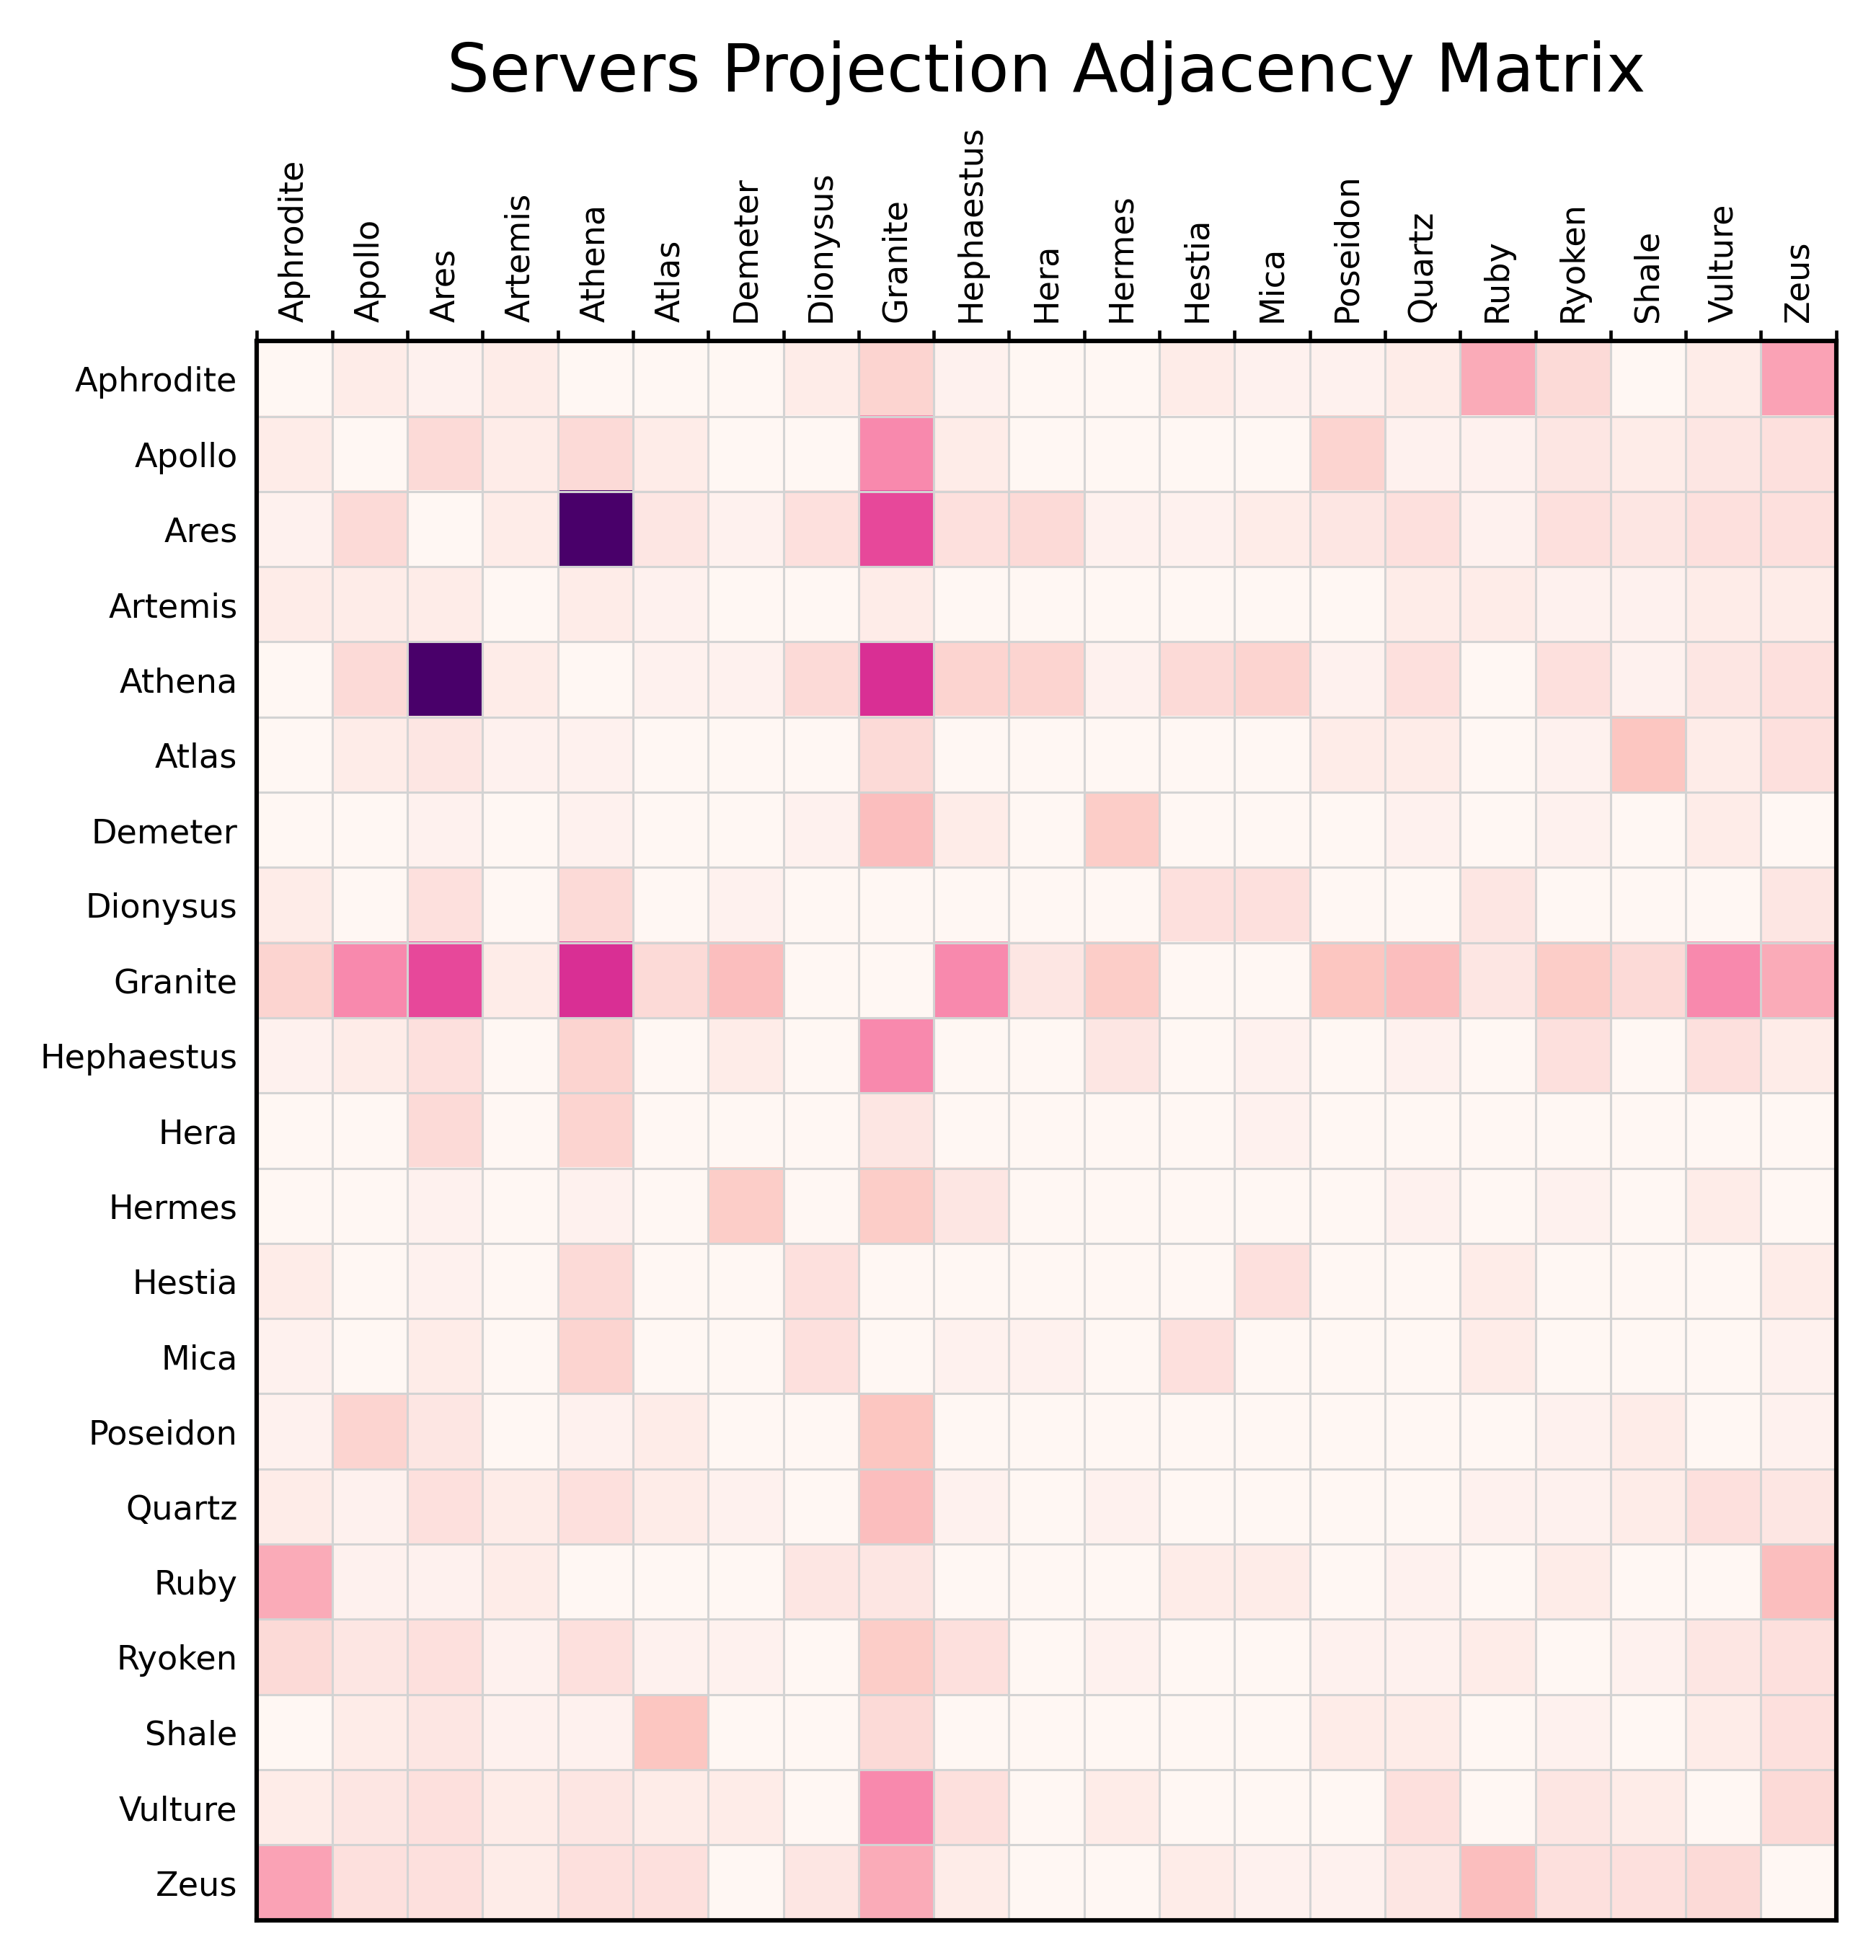
\includegraphics[height=0.24\textheight]{../res/Adjacency_Matrix_Servers.png}
        \caption{Server projection.}
        \label{fig:server-adjacency}
    \end{subfigure}
    \caption{Original connection matrix and weighted adjacency matrices. White cells indicate no edge; darker cells indicate stronger shared-connection weights.}
    \label{fig:matrices}
\end{figure}

\subsection{Visual Exploration}

The server graph is easier to inspect visually because it has fewer nodes. The computer graph is denser, so visual exploration is combined with numerical measures.

\section{Centrality and Influential Nodes}

\subsection{Centrality Measures}

Three centrality measures are computed: degree, closeness, and betweenness centrality. They respectively measure direct connectivity, reachability, and bridge-like behavior.

Since they capture different types of influence, the full centrality tables are reported in the notebook and interpreted together. In the report, the discussion focuses on the nodes that are strongest under the weighted projection, because edge weights represent the intensity of shared connections.

\subsection{Most Influential Servers}

By weighted connectivity, the strongest servers are Granite, Athena, and Ares. Granite has the largest total shared-connection strength, while Ares and Athena also appear as central servers in the projected structure. The strongest server-server relationship is Ares--Athena, which reinforces their role in the graph.

\subsection{Most Influential Computers}

By weighted degree, the strongest computers are 12, 119, 55, 78, 152, 121, 117, 126, 149, and 108. These nodes are the most involved in repeated shared-server relationships.

\subsection{Observation}

An interesting observation is that influence appears more concentrated in the server graph. The strongest server edges have much larger weights than the strongest computer edges, suggesting stronger shared usage among servers than among individual computers.

\section{Community Detection}

\subsection{Method}

To identify communities, two algorithms are applied to both projected graphs: Louvain and Girvan-Newman. The goal is to detect groups of nodes that are more strongly connected internally than with the rest of the graph. Each community is then represented in the plots using a different color.

Using both algorithms on both graphs makes the comparison more informative. The two methods are based on different ideas: Louvain searches for a partition that improves modularity, while Girvan-Newman progressively removes edges that are likely to connect different communities. Therefore, they do not necessarily produce the same structure, especially when the graph is dense.

\subsection{Comparison Between Algorithms}

Louvain produced a more readable partition for the computer graph. This graph is larger and denser, so a modularity-based method gives a useful summary of its structure. Instead of trying to visually follow many individual edges, Louvain groups computers according to the overall strength of their shared-server relationships.

Girvan-Newman was easier to interpret visually on the server graph. Since the server graph has fewer nodes, the progressive removal of bridging edges is more visible. The smaller size makes it clearer which connections separate one group of servers from another.

This does not mean that one algorithm is universally better. The difference is mainly caused by the size and density of the two projected graphs. The server graph is compact enough for Girvan-Newman to expose separations clearly, while the computer graph benefits from an algorithm that summarizes a larger and more connected structure.

\subsection{Analysis}

The community results show that both projections contain internal structure. In the server graph, communities correspond to groups of servers that tend to be used by similar sets of computers. In the computer graph, communities correspond to groups of computers that share similar server usage patterns.

The server communities are easier to interpret visually because the graph contains only 21 nodes. The community colors reveal groups of servers that are close to each other in the projected graph, and the separation between groups is more visible. This makes the server graph a good case for interpreting the qualitative behavior of the algorithms.

The computer graph is more difficult to interpret from the plot alone. It contains many more nodes and many shared relationships, so the drawing is naturally denser. In this case, the community assignment is more useful as a structural summary than as a purely visual result. Louvain gives a clearer view of this structure by grouping nodes according to modularity, as shown in Figure~\ref{fig:computer-louvain}.

Overall, the community detection step confirms that the dataset is not just a uniform collection of connections. Both graphs contain groups of nodes with stronger internal similarity, but the best way to observe this structure depends on the graph. The full visual comparison of both algorithms on both graphs is included in the notebook.

\section{Largest Clique}

\subsection{Method}

The next step is to identify the largest clique in each projected graph. A clique is a set of nodes where every node is directly connected to every other node in the same set. In the context of this project, this gives a very strict notion of similarity.

In the server graph, a clique represents a group of servers where every pair of servers shares at least one computer. In the computer graph, a clique represents a group of computers where every pair of computers shares at least one server. This is stronger than community detection: a community only needs to be densely connected, while a clique must be fully connected.

After identifying the largest clique, the graph is plotted again with the clique nodes highlighted using a different color. This makes it possible to see where the fully connected group is located inside the larger graph structure. The complete visualizations are included in the notebook.

\subsection{Analysis}

The largest clique in the server graph has size 11. Since the server graph contains 21 nodes, this is a substantial result: more than half of the servers belong to a group in which every server is connected to every other server in the group. This indicates that there is a core set of servers with strong shared usage patterns.

The largest clique in the computer graph has size 69. This is also an important result because it shows that a large subset of computers is pairwise connected through shared servers. The computers in this clique do not necessarily have identical server connections, but every pair of them shares at least one server.

The size of the computer clique also explains why the computer graph appears dense and difficult to interpret visually. A clique of 69 nodes creates many pairwise relationships, so the graph contains a large highly connected region. In this case, the clique analysis is more informative than the raw plot alone, because it identifies the exact presence of a fully connected structure. The highlighted clique is shown in Figure~\ref{fig:computer-clique}.

\begin{figure}[h]
    \centering
    \begin{subfigure}{0.49\textwidth}
        \centering
        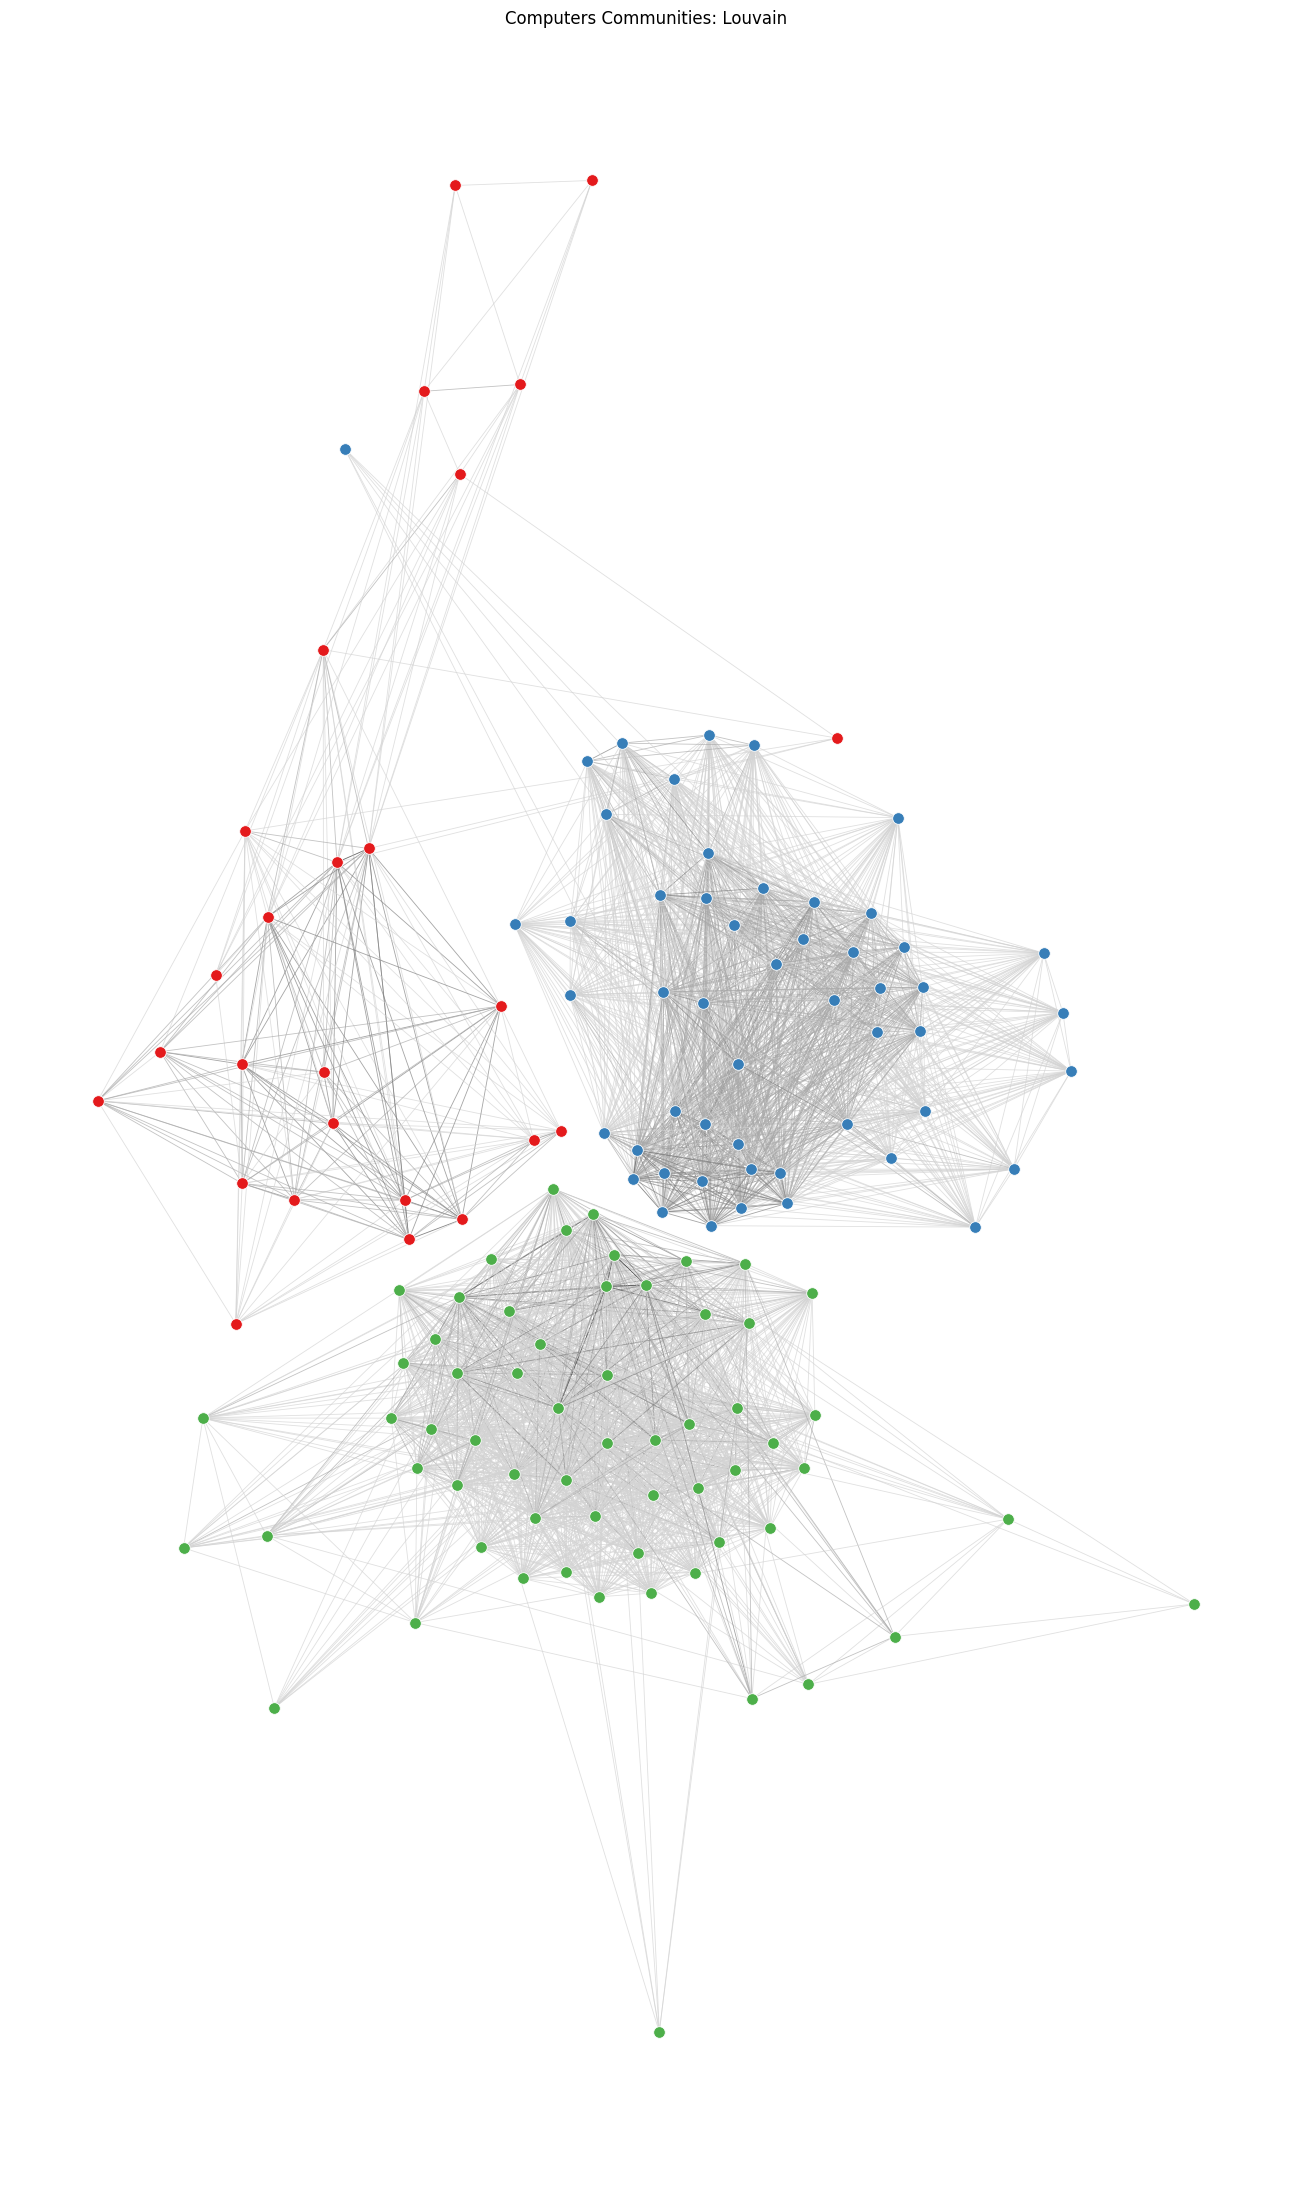
\includegraphics[width=\textwidth]{../res/Communities_Computers_Louvain.png}
        \caption{Louvain communities.}
        \label{fig:computer-louvain}
    \end{subfigure}
    \hfill
    \begin{subfigure}{0.49\textwidth}
        \centering
        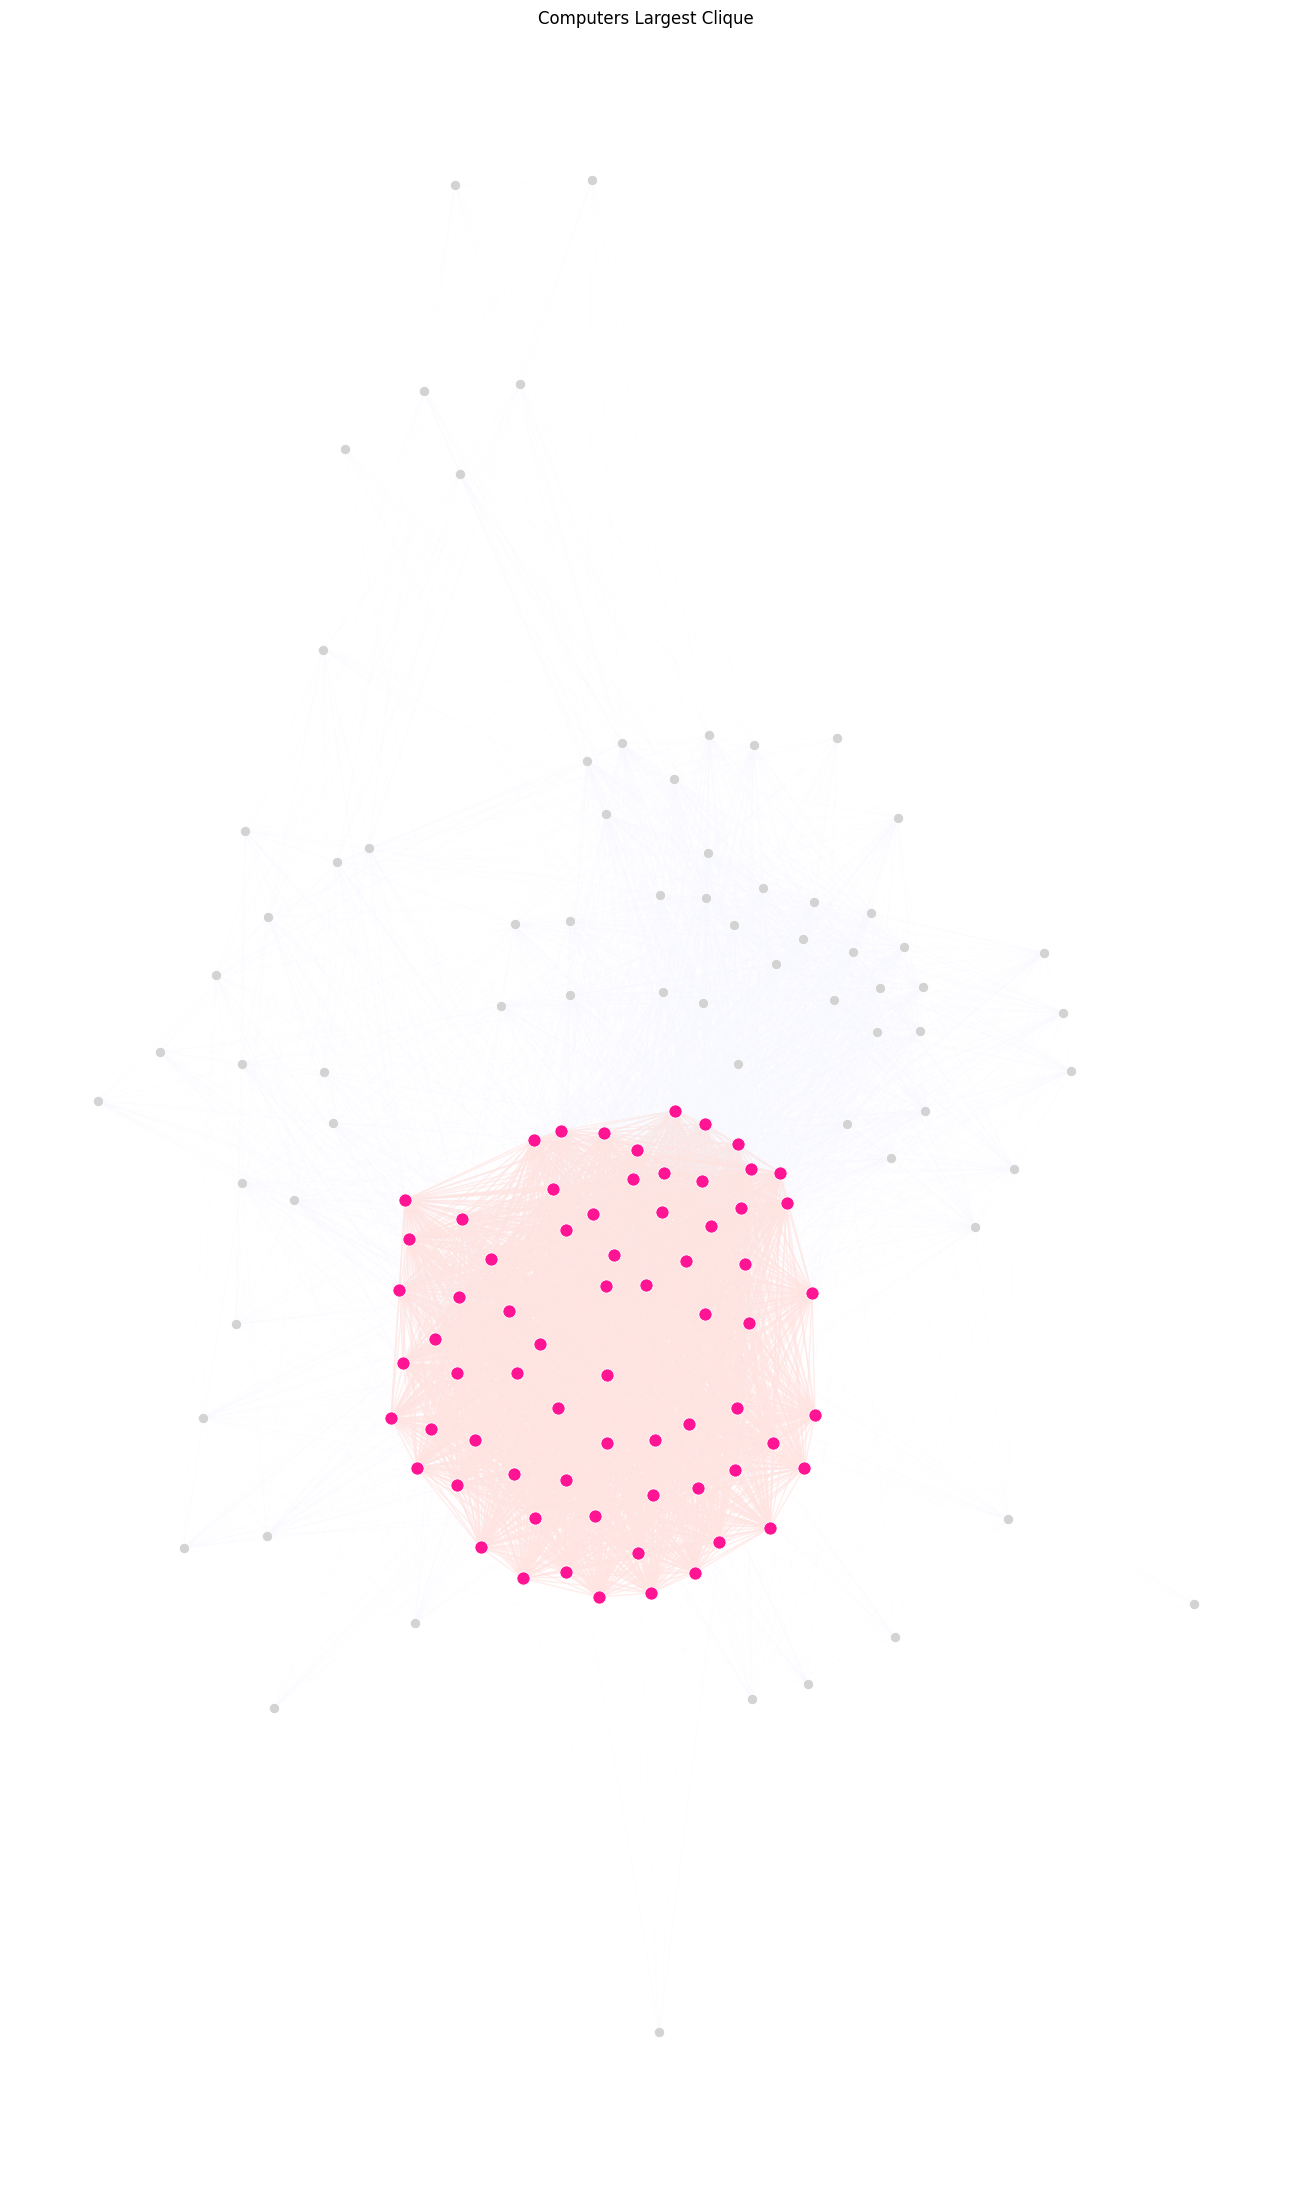
\includegraphics[width=\textwidth]{../res/Largest_Clique_Computers.png}
        \caption{Largest clique.}
        \label{fig:computer-clique}
    \end{subfigure}
    \caption{Computer projection: community structure and largest clique.}
    \label{fig:computer-structure}
\end{figure}

\subsection{Interpretation}

The clique results complement the community results. Communities describe groups with relatively strong internal connectivity, while cliques identify the strictest possible form of internal connectivity. The large server clique suggests a central group of servers that are mutually related through common computers. The large computer clique suggests that many computers share at least one server with each other, creating a broad core of pairwise overlap.

Therefore, the largest clique analysis confirms that the dataset contains not only loose communities, but also highly cohesive substructures. These structures are especially relevant because they are derived directly from shared connections in the original matrix.

\section{Heavy Hitters}

\subsection{Definition}

The final task is to identify heavy hitters. Since the projected graphs are weighted, the definition should take edge weights into account. For this reason, heavy hitters are identified using weighted degree rather than ordinary degree.

The weighted degree of a node is the sum of the weights of all edges incident to that node. This measure captures both how many relationships a node has and how strong those relationships are. A node connected to many others through weak overlaps is therefore distinguished from a node involved in several strong shared-connection patterns.

In this analysis, a node is considered a heavy hitter if it belongs to the top ten nodes by weighted degree in its graph. With this definition, the minimum weighted degree for a server to be considered a heavy hitter is 38. The minimum weighted degree for a computer to be considered a heavy hitter is 173.

\subsection{Server Heavy Hitters}

The server heavy hitters are Granite, Athena, Ares, Zeus, Apollo, Vulture, Aphrodite, Hephaestus, Ryoken, and Quartz. Granite is the strongest server, with a weighted degree of 157. Athena and Ares follow with weighted degrees of 109 and 104.

These values show that the server graph has a small group of highly central nodes. Granite is especially important because it has the largest total amount of shared usage with other servers. The presence of Ares and Athena among the top nodes is consistent with the earlier observation that Ares--Athena is the strongest server-server edge.

\subsection{Computer Heavy Hitters}

The computer heavy hitters are 12, 119, 55, 78, 152, 121, 117, 126, 149, and 108. Computer 12 is the strongest computer, with a weighted degree of 199. The remaining heavy hitters have weighted degrees between 173 and 188.

These computers are the most involved in shared-server relationships. Their weighted degree values indicate that they are not only connected to other computers, but that these connections are supported by repeated server overlap.

\subsection{Interpretation}

The heavy hitter analysis confirms that the strongest activity is not evenly distributed. A relatively small set of servers and computers accounts for the strongest weighted relationships in the projected graphs.

The comparison between the two graphs is also informative. The top server edges have higher weights than the top computer edges, which suggests that server overlap is more concentrated. In other words, some pairs of servers are shared by many computers, while pairs of computers generally share fewer servers.

This result is consistent with the rest of the analysis: the server graph contains a compact group of highly influential nodes, while the computer graph is larger, denser, and better understood through aggregate measures such as weighted degree, communities, and clique size.

\section{Conclusion}

This project shows how the original computer-server connection matrix can be transformed into graph representations that reveal different structural properties of the data. By constructing both the computer projection and the server projection, the analysis captures two complementary perspectives: similarity between computers based on shared servers, and similarity between servers based on shared computers.

The exploratory analysis shows that the two projections behave differently. The server graph is smaller and more visually interpretable, while the computer graph is larger and denser. For this reason, the report combines visual inspection with centrality measures, community detection, clique analysis, and weighted-degree rankings.

Across the analyses, the server graph shows a more concentrated structure. Servers such as Granite, Athena, and Ares appear repeatedly as influential nodes, and the strongest server-server relationships have high weights. The computer graph, on the other hand, contains a large clique and a broad dense structure, making aggregate measures particularly useful for interpretation.

Overall, the analysis demonstrates that graph-based methods can reveal meaningful structure in connection data. The combination of centrality measures, community detection, clique analysis, and weighted-degree rankings provides complementary perspectives on influence, cohesion, and similarity within the network.

One limitation of this analysis is that the projected graphs reduce the original computer-server structure into one-mode networks, which may hide some information about the exact computer-server relationships.

\end{document}
